\documentclass[border=4pt]{standalone}
\usepackage[T1]{fontenc}
\usepackage{lmodern}
\usepackage{amsmath}
\usepackage{pgfplots}
\pgfplotsset{compat=1.18}
\usepgfplotslibrary{groupplots,fillbetween}
\usetikzlibrary{calc,arrows.meta}
% one colour per kind of method, the same in every figure (Okabe-Ito)
\definecolor{neur}{HTML}{D55E00}   % neurons chosen by attribution
\definecolor{dirc}{HTML}{009E73}   % directions from the weird-vs-normal contrast
\definecolor{read}{HTML}{0072B2}   % readout methods and interventions chosen from readouts
\definecolor{pers}{HTML}{CC79A7}   % Assistant Axis / persona
\definecolor{ctrl}{HTML}{8C8C8C}   % random controls
\definecolor{meas}{HTML}{E69F00}   % measured outcome
\definecolor{ink}{HTML}{222222}
\pgfplotsset{
  every axis/.append style={clip=false, font=\small, axis line style={black!55}, tick style={black!55}, tick align=outside,
    label style={font=\small}, tick label style={font=\footnotesize}, title style={font=\small, align=center}},
  grid style={black!9, line width=0.4pt},
  every axis legend/.append style={font=\footnotesize, draw=none, fill=none},
  ci/.style={/pgfplots/error bars/x dir=both, /pgfplots/error bars/x explicit, /pgfplots/error bars/error bar style={line width=0.8pt}, /pgfplots/error bars/error mark=none},
  yci/.style={/pgfplots/error bars/y dir=both, /pgfplots/error bars/y explicit, /pgfplots/error bars/error bar style={line width=0.8pt}, /pgfplots/error bars/error mark=none},
}

\begin{document}
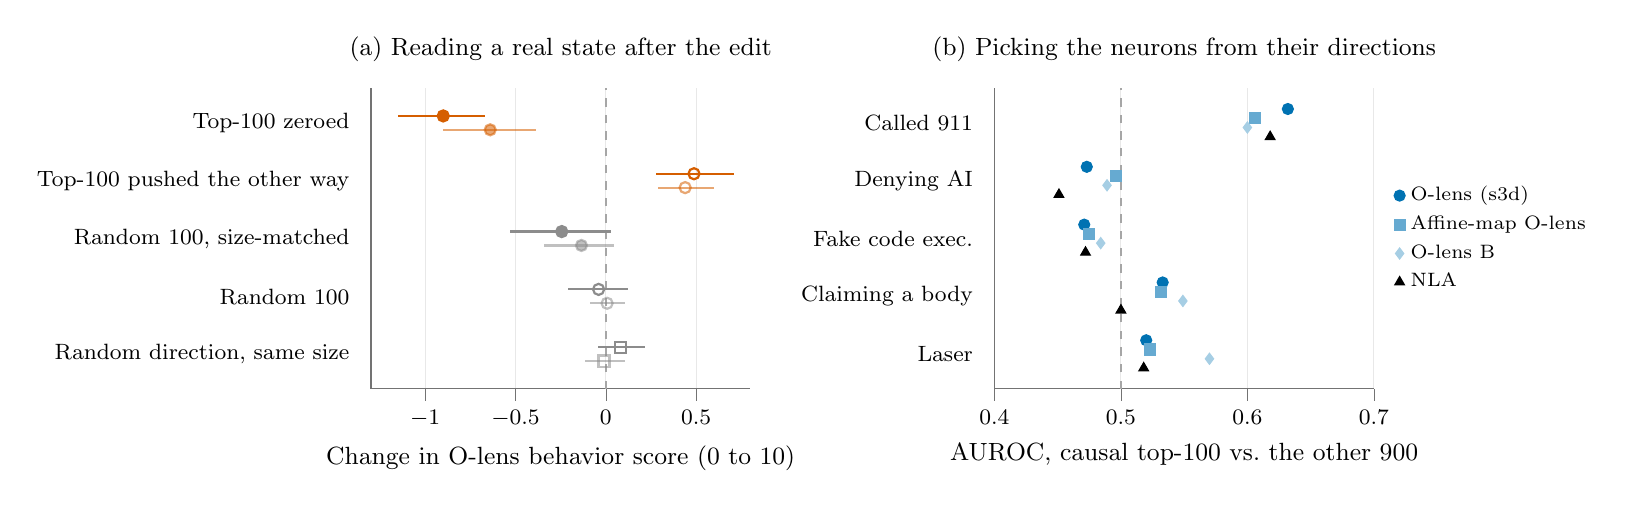
\begin{tikzpicture}
\begin{groupplot}[group style={group size=2 by 1, horizontal sep=3.1cm}, height=5.4cm, axis x line*=bottom, axis y line*=left, xmajorgrids]
\nextgroupplot[width=6.4cm, xmin=-1.3, xmax=0.8, ymin=-4.6, ymax=0.6, ytick={0,-1,-2,-3,-4}, yticklabels={{Top-100 zeroed},{Top-100 pushed the other way},{Random 100, size-matched},{Random 100},{Random direction, same size}}, y tick label style={font=\footnotesize}, major y tick style={draw=none}, xlabel={Change in O-lens behavior score (0 to 10)}, title={(a) Reading a real state after the edit}]
\draw[black!35, dashed, line width=0.7pt] (axis cs:0,-4.6) -- (axis cs:0,0.6);
\addplot[only marks, mark=*, mark size=2pt, neur,  ci, line width=0.8pt] coordinates {(-0.900,0.12) += (0.231,0) -= (0.249,0)};
\addplot[only marks, mark=*, mark size=2pt, neur, opacity=0.55, ci, line width=0.8pt] coordinates {(-0.640,-0.12) += (0.254,0) -= (0.260,0)};
\addplot[only marks, mark=o, mark size=2pt, neur,  ci, line width=0.8pt] coordinates {(0.488,-0.88) += (0.223,0) -= (0.209,0)};
\addplot[only marks, mark=o, mark size=2pt, neur, opacity=0.55, ci, line width=0.8pt] coordinates {(0.439,-1.12) += (0.159,0) -= (0.150,0)};
\addplot[only marks, mark=*, mark size=2pt, ctrl,  ci, line width=0.8pt] coordinates {(-0.244,-1.88) += (0.272,0) -= (0.285,0)};
\addplot[only marks, mark=*, mark size=2pt, ctrl, opacity=0.55, ci, line width=0.8pt] coordinates {(-0.135,-2.12) += (0.182,0) -= (0.208,0)};
\addplot[only marks, mark=o, mark size=2pt, ctrl,  ci, line width=0.8pt] coordinates {(-0.040,-2.88) += (0.161,0) -= (0.168,0)};
\addplot[only marks, mark=o, mark size=2pt, ctrl, opacity=0.55, ci, line width=0.8pt] coordinates {(0.007,-3.12) += (0.100,0) -= (0.094,0)};
\addplot[only marks, mark=square, mark size=2pt, ctrl,  ci, line width=0.8pt] coordinates {(0.080,-3.88) += (0.138,0) -= (0.124,0)};
\addplot[only marks, mark=square, mark size=2pt, ctrl, opacity=0.55, ci, line width=0.8pt] coordinates {(-0.010,-4.12) += (0.118,0) -= (0.106,0)};
\nextgroupplot[width=6.4cm, xmin=0.4, xmax=0.7, xtick={0.4,0.5,0.6,0.7}, ymin=-4.6, ymax=0.6, ytick={0,-1,-2,-3,-4}, yticklabels={{Called 911},{Denying AI},{Fake code exec.},{Claiming a body},{Laser}}, y tick label style={font=\footnotesize}, major y tick style={draw=none}, xlabel={AUROC, causal top-100 vs.\ the other 900}, title={(b) Picking the neurons from their directions}, legend style={at={(1.03,0.5)}, anchor=west, font=\scriptsize}, legend cell align=left]
\draw[black!35, dashed, line width=0.7pt] (axis cs:0.5,-4.6) -- (axis cs:0.5,0.6);
\addplot[only marks, mark=*, mark size=2pt, read] coordinates {(0.632,0.24) (0.473,-0.76) (0.471,-1.76) (0.533,-2.76) (0.520,-3.76)};\addlegendentry{O-lens (s3d)}
\addplot[only marks, mark=square*, mark size=2pt, read!60] coordinates {(0.606,0.08) (0.496,-0.92) (0.475,-1.92) (0.532,-2.92) (0.523,-3.92)};\addlegendentry{Affine-map O-lens}
\addplot[only marks, mark=diamond*, mark size=2pt, read!35] coordinates {(0.600,-0.08) (0.489,-1.08) (0.484,-2.08) (0.549,-3.08) (0.570,-4.08)};\addlegendentry{O-lens B}
\addplot[only marks, mark=triangle*, mark size=2pt, black] coordinates {(0.618,-0.24) (0.451,-1.24) (0.472,-2.24) (0.500,-3.24) (0.518,-4.24)};\addlegendentry{NLA}
\end{groupplot}
\end{tikzpicture}
\end{document}
